\documentclass[11pt]{article}
\usepackage{fullpage}
\usepackage{amsmath}
\usepackage{mathtools}
\usepackage{esint}
\usepackage{cancel}
\usepackage{graphicx}
\usepackage{xcolor}
\usepackage{float}
\linespread{1.1}
\allowdisplaybreaks
\usepackage{color}
\usepackage{listings}
\usepackage{subfigure}
\usepackage{xcolor}
\usepackage{sectsty}
\definecolor{darkblue}{RGB}{10,0,100}
\definecolor{otherblue}{RGB}{0,70,200}
\sectionfont{\color{darkblue}} 
\subsectionfont{\color{otherblue}}  

\begin{document}

\title{APS360  \\ Applied Fundamentals of Machine Learning}
\author{Michael Boyadjian}
\maketitle
\pagebreak

\tableofcontents

\pagebreak

\bigskip
\bigskip
\bigskip

\section{Introduction to Machine Learning}
 \hrule \vspace{15pt}

\subsection{Terminology}
\begin{itemize}
\item \textbf{Artificial Intelligence}
\begin{itemize}
\item The intelligence of machines and the branch of computer science that aims to create it.
\item The science and engineering of making intelligent machines, especially intelligent computer programs.
\item Often used to describe machines (or computers) that mimic "cognitive" functions that humans associate with the human mind, such as "learning" and "problem solving".
\item \textit{Create intelligent machines that work and act like humans.}
\end{itemize}
\item \textbf{Machine Learning}
\begin{itemize}
\item A branch of artificial intelligence concerned with design and development of algorithms to build mathematical models based on sample data, known as "training data", in order to make predictions or decisions without being explicitly programmed to perform the task
\item \textit{Find an algorithm that automatically learns from structured (preprocessed) example data.}
\end{itemize}
\item \textbf{Deep Learning}
\begin{itemize}
\item Deep learning is a subset of machine learning that has networks capable of learning unsupervised from data that is unstructured or unlabeled. Also known as deep neural learning or deep neural network.
\item \textit{Uses deep neural networks to automatically learn from unstructured example data.}
\end{itemize}
\end{itemize}

\subsection{AI Reality}
\begin{itemize}
\item AI works well on pattern recognition problems with big data  ; examples include voice recognition, facial recognition, etc.
\item AI does not work as well on on planning and prediction; examples include stock market, language, comedy, etc.
\end{itemize}

\subsection{Types of Learning}
\begin{itemize}
\item \textbf{Supervised Learning}
\begin{itemize}
\item Learning model that maps an input to an output based on example input-output pairs \textit{(ex. age prediction given a headshot)}
\item Machine learning is a game of balance, with our objective being to generalize to all possible future data
\end{itemize}
\item \textbf{Unsupervised Learning}
\begin{itemize}
\item Focuses on finding patterns, regularities or structure in (unlabeled) data \textit{(ex. clustering,  style transfer, etc.)}
\end{itemize}
\item \textbf{Reinforcement Learning}
\begin{itemize}
\item Learning what actions to take to optimize long-term reward \textit{(ex. playing a video game,  learning to walk, etc.)}
\item Correct input/label pairs are never presented, nor are sub-optimal actions explicitly corrected
\item Payoff is often delayed
\end{itemize}
\end{itemize}

\subsection{Data Splitting}
\begin{itemize}
\item \textbf{Training and Testing Data}
\begin{itemize}
\item More data leads to a better model, but we need to set some aside for testing
\item Have a training and testing split
\item Trying until favourable outcomes are achieved would make testing data effectively same as training data and would lead to overfitting
\end{itemize}
\item \textbf{Validation and Holdout Data}
\begin{itemize}
\item Split the testing data into validation and holdout
\item Only use holdout data once
\item Typical splits are $60/20/20$, $70/15/15$,  or $80/10/10$
\end{itemize}
\end{itemize}


\pagebreak



\section{Artificial Neural Networks (ANNs)}
\hrule \vspace{15pt}

\subsection{Biological Neurons}
\subsubsection{Artificial Pigeon}
In order to use an artificial neural network (pigeon) to solve a simple classification problem, we will need to:
\begin{enumerate}
\item Build an artificial neural network -- or rather,  an artificial (pigeon) brain
\item Decide how to reward the artificial pigeon
\item Decide how to train the artificial pigeon
\item Determine how well our artificial pigeon performs the classification task
\end{enumerate}
\subsubsection{Neuron Anatomy}
\begin{itemize}
\item The \textbf{dendrites}, which are connected to other cells that provides information.
\item The \textbf{cell body} (soma), which consolidates information from the dendrites.
\item The \textbf{axon}, which is an extension from the cell body that passes information to other cells.
\item The \textbf{synapse}, which is the area where the axon of one neuron and the dendrite of another connect.
\begin{itemize}
\item Small voltage difference between inside and outside of cell
\item When a neuron receives “information” in its dendrites, the voltage difference along that part of the cell lowers.
\item If the total activity in a neuron’s dendrites lowers the voltage difference enough, the entire cell depolarizes and the cell fires.
\item The voltage signal spread along the axon and to the synapse, then to the next cells.
\end{itemize}
\end{itemize}
\begin{center}
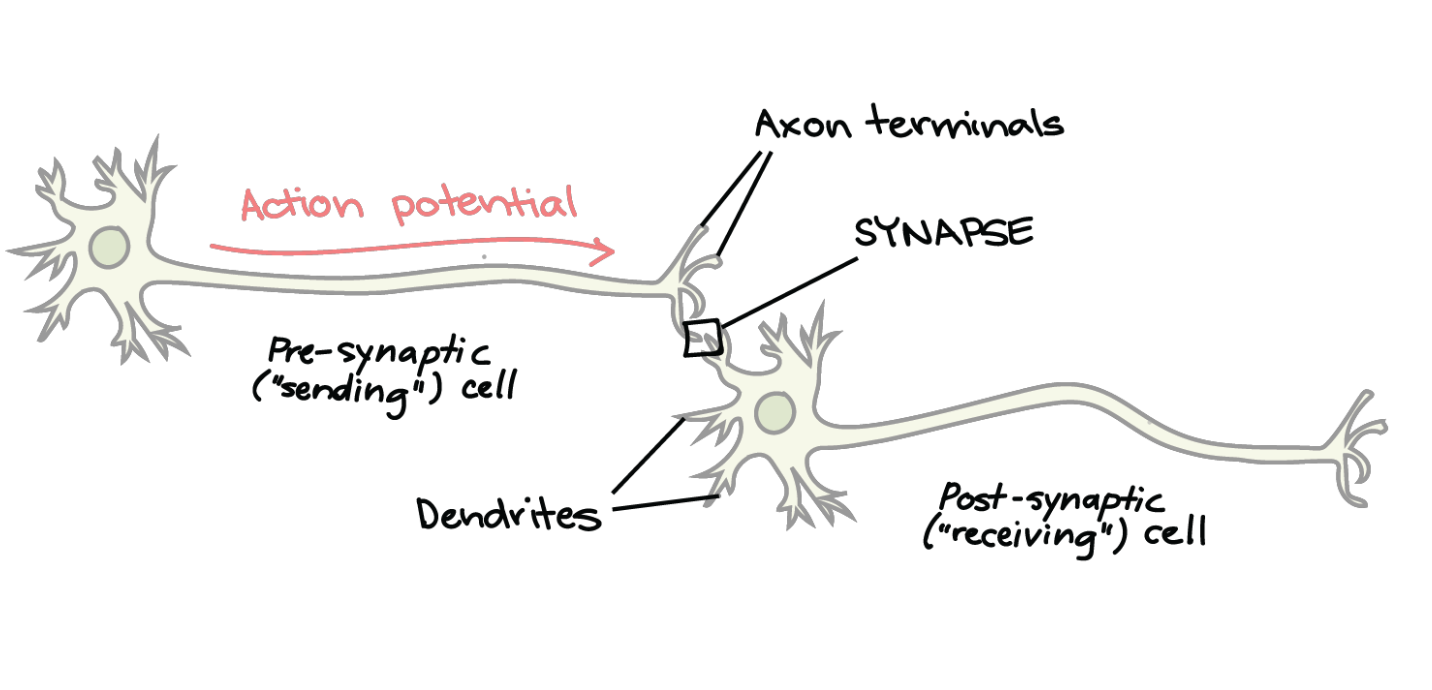
\includegraphics[scale=0.55]{images/synapse.png}
\end{center}



\subsection{Artificial Neurons}
\begin{itemize}
\item Here the neuron is actually a processing unit, it calculates the weighted sum of the input signal to the neuron to generate the activation signal $v_k$
$$ v_k = \sum_{i=0}^p w_i x_i = w^Tx$$
\item Then a hard threshold is applied on the activation signal to get the output signal $y_k$
\item $x_0$ is reserved for the bias
\end{itemize}
\begin{center}
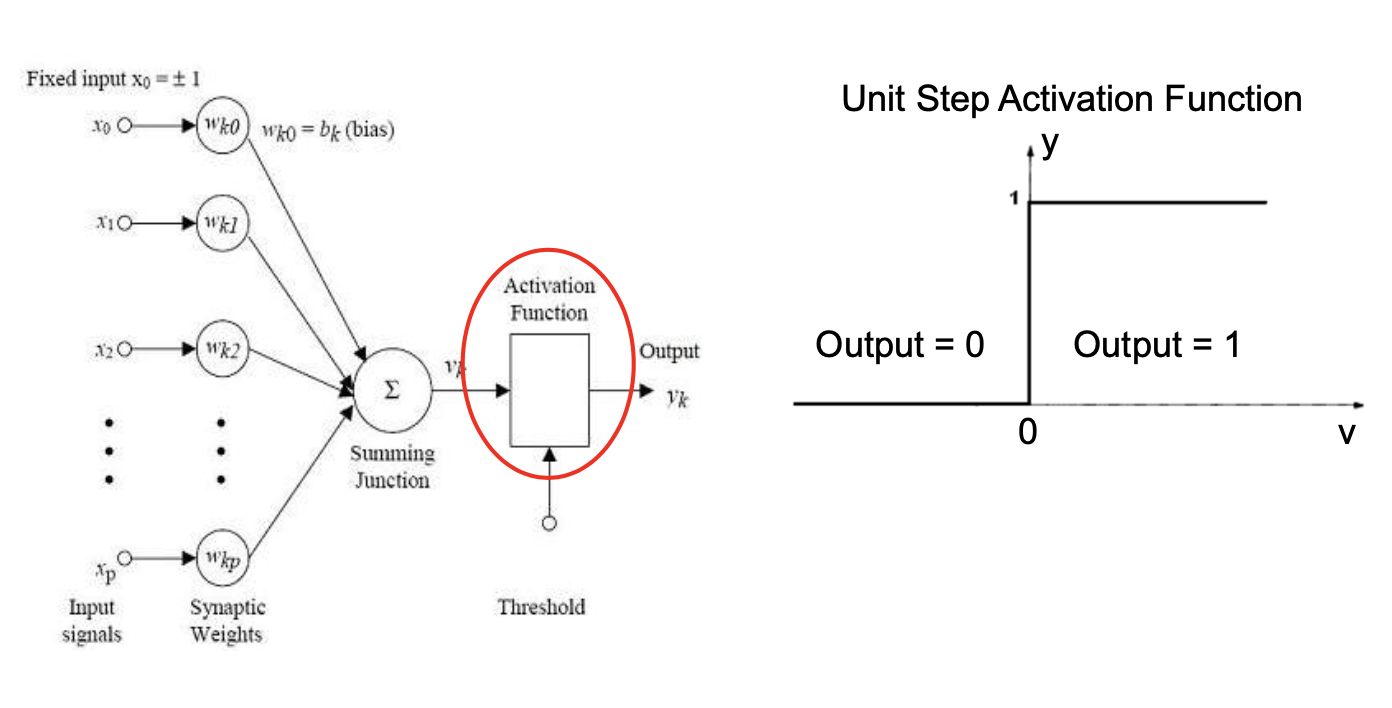
\includegraphics[scale=0.58]{images/artneuron.png}
\end{center}
\subsection{Forward Pass}
\subsubsection{Error}
In order to train an ANN we first have to define the error on our classifications (loss function),  the error depends on the problem.  For \textbf{regression} problems we use mean squared error (MSE):
$$ MSE = \frac{1}{N} \sum_{n=1}^N (y_i - t_i)^2 $$
where $N$ is the number of training samples, $y$ is the model predicted output and $t$ is the desired output. For \textbf{classification} problems we use cross entropy (CE):
$$ CE = -\frac{1}{N} \sum_{n=1}^N \sum_{k=1}^K t_{n,k} \log (y_{n,k}) $$ 
where $N$ is the number of training samples, $K$ is the number of classes, $y$ is the model predicted output and $t$ is the target label. The objective is to get $error \approx 0$.
\subsubsection{Weight Tuning}
\begin{itemize}
\item Randomly pick weights until it works 
\item Change one weight at a time in the direction that reduces error
\item Gradient descent - Adjusting weights according to the slope (gradient) will guide us to the minimum error
\begin{center}
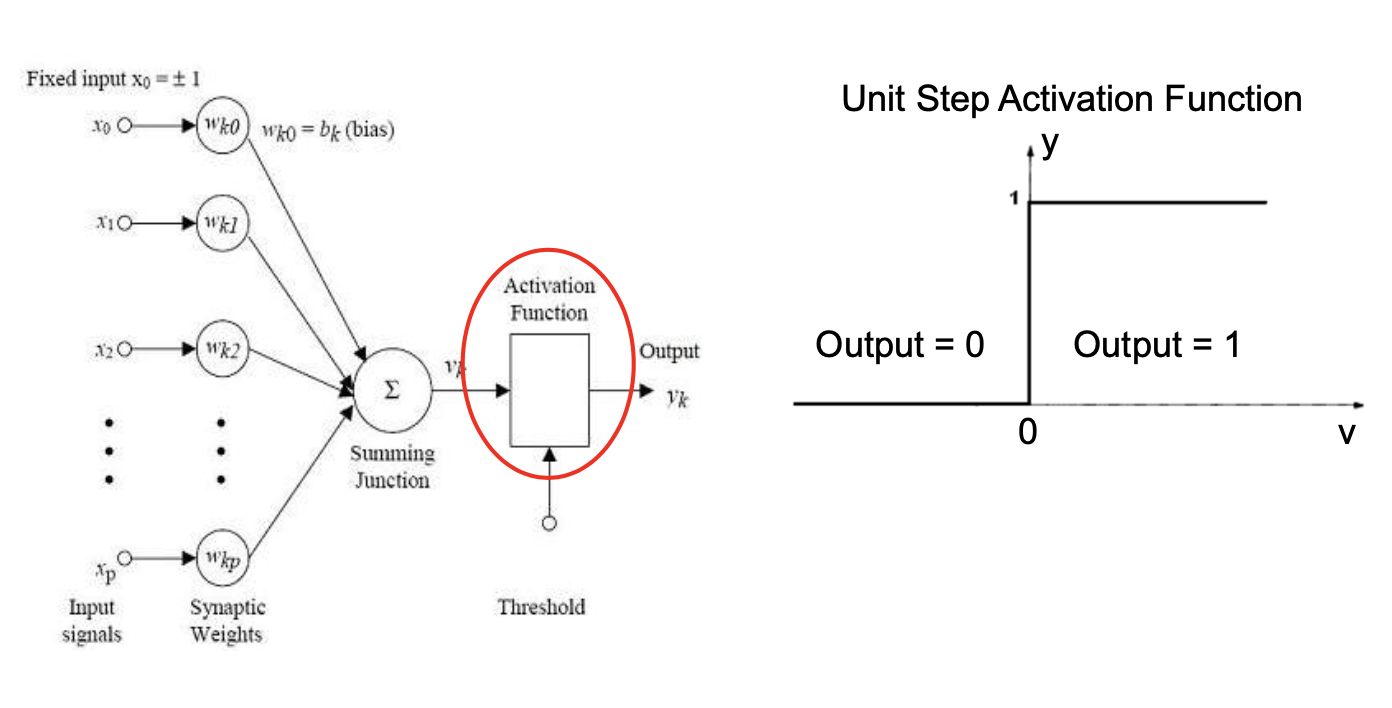
\includegraphics[scale=0.4]{images/artneuron.png}
\end{center}
\end{itemize}


\subsection{Back Propagation}
\subsubsection{Gradient Descent }
\begin{itemize}
\item Find how the error changes as you change each weight ($\frac{dE}{dw}$)
\item Update weight in the opposite direction of the gradient 
$$ W = W - \eta \frac{dE}{dW}$$ 
where $\eta$ is the learning rate,  the step size taken according to the gradient 
\item Need the function be differentiable
\item Step function gradient undefined at $f(0$), and $0$ everywhere else,  require another activation function - we can use sigmoid (logistic) activation function 
\end{itemize}
\begin{center}
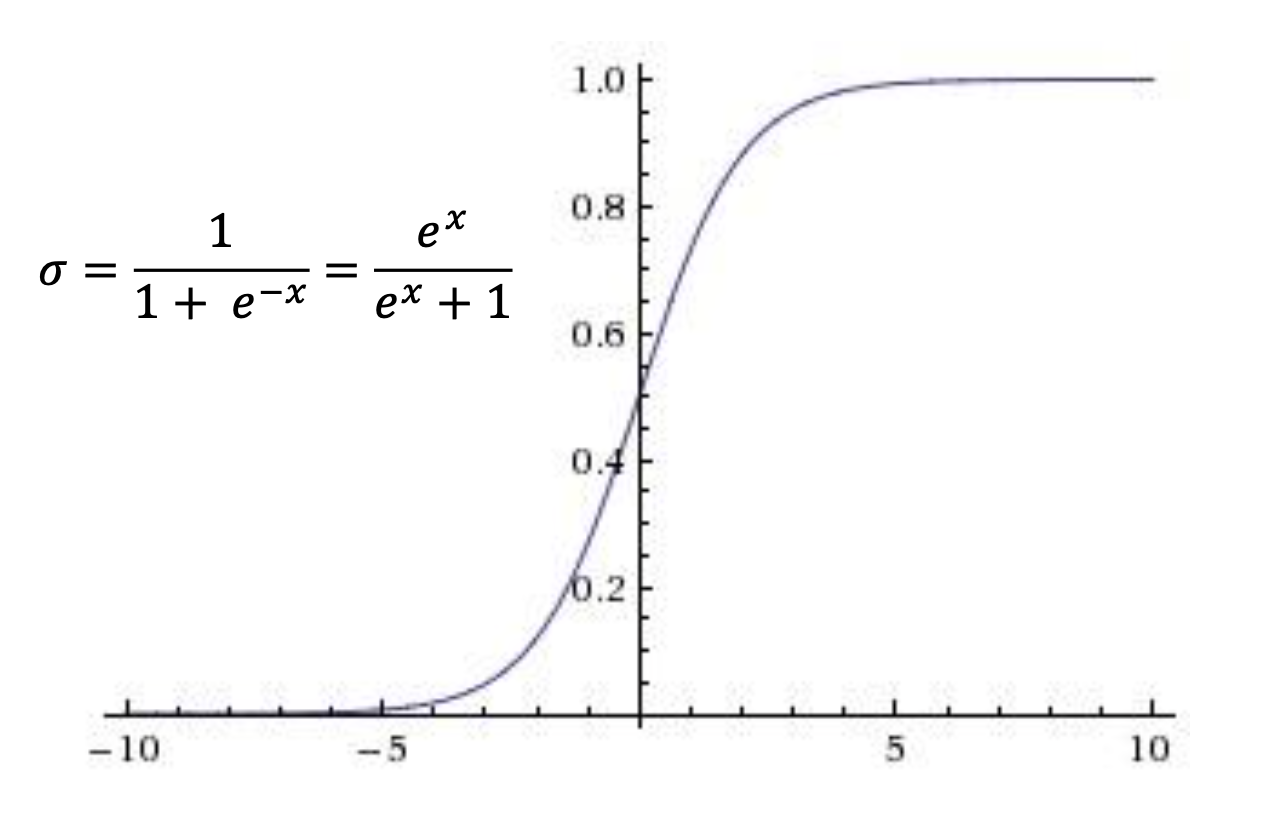
\includegraphics[scale=0.35]{images/sigmoid.png}
\end{center}
\begin{itemize}
\item Other activation functions include $\tanh$ activation and $ReLU$ activation
$$ tanh = \frac{e^x - e^{-x}}{e^x + e^{-x}} = \frac{e^{2x} -  1}{e^{2x} + 1} $$ 
$$ ReLU = \max \{ 0,  x \} $$ 
\item $ReLU$ is a preferred activation function
\begin{itemize}
\item Resolves vanishing gradients issues resulting from deep networks
\item Computationally more efficient
\end{itemize}
\end{itemize}

\subsection{ANN Architecture}
\begin{itemize}
\item An architecture of a neural network describes the neurons and their connectivity in the network
\item Information only flows from one layer to a later layer, from the input to the output.
\item Neurons between adjacent layers are fully pairwise connected.
\item Input layer is not counted in number of layers 
\end{itemize}
\begin{center}
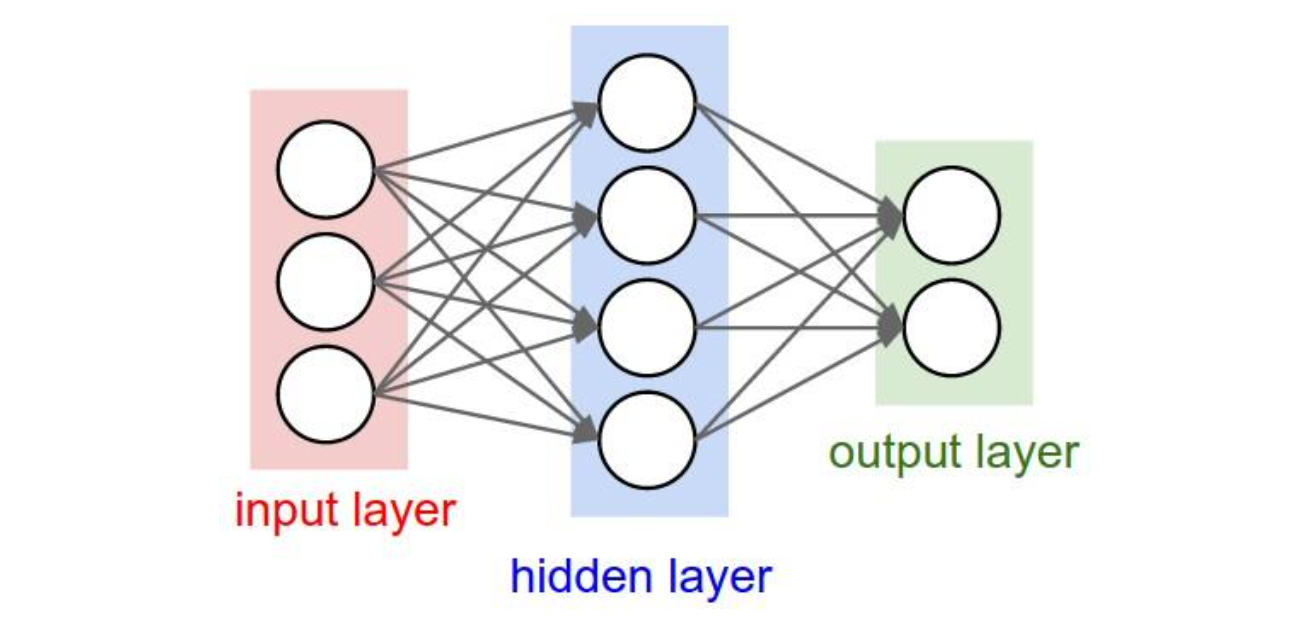
\includegraphics[scale=0.5]{images/ann.png}
\end{center}
\begin{itemize}
\item Adding more linear layers does not help increase the capacity of the model
\item Any sequence of linear layers can be equivalently represented with a single linear layer.
\end{itemize}

\subsection{ANN Training}
Training deals with techniques for effectively and efficiently tuning the model weights (parameters). To train we need to calculate the error on the predictions (classifications), which we can achieve with a Loss Function. An optimizer is then used to achieve this more efficiently
\subsubsection{Loss Function}
\begin{itemize}
\item Computes how “bad” a set of predictions was, compared to the ground truth (labels).
\begin{itemize}
\item \textbf{Large loss} = the network’s prediction differs from the ground truth
\item \textbf{Small loss} = the network’s prediction matches the ground truth
\end{itemize}
\end{itemize}
\subsubsection{Optimizer}
\begin{itemize}
\item An optimizer determines, based on the value of the loss function, how each parameter (weight) should change.
\item Solves the credit assignment problem: how do we assign credit (blame) to the parameters based on how the network performs?
\item Each update of the weights takes one step towards solving the optimization problem
\item We use the derivative of the loss function at a training example, and take a step towards its negative gradient
\end{itemize}
\subsubsection{Forward and Backward Pass}
\begin{itemize}
\item\textbf{Forward Pass}
\begin{itemize}
\item Makes a prediction
\item Information flows forwards from input to
output layer
\end{itemize}
\item \textbf{Backward Pass}
\begin{itemize}
\item Computes gradients for making changes to weights
\item Information flows backwards from output to input layer
\end{itemize}
\end{itemize}

\subsection{Hyperparameter Tuning}
Hyperparameters are neural network settings that cannot be optimized using an optimizer
\subsubsection{Batch Size}
\begin{itemize}
\item Instead of working with one sample at a time we apply batching:
\begin{enumerate}
\item Use our network to make the predictions for n images
\item Compute the average loss for those n images
\item Take a “step” to optimize the average loss of those n images
\end{enumerate}
\item The batch size is the number of training examples used per optimization “step”.
\item Each optimization “step” is known as an iteration.
\item The parameters are updated once per iteration.
\item If batch size\textbf{ too small} = we optimize a (possibly very) different function; noisy
loss at each iteration
\item If batch size \textbf{too large} = average loss might not change very much as batch size grows; expensive
\end{itemize}
\subsubsection{Epochs}
\begin{itemize}
\item An epoch is a measure of the number of times all training data are used once to update the parameters.
\item \textbf{example}: 1000 images for training $\rightarrow$ uf $batchsize = 10$ then $100 \; iterations = 1 \; epoch$
\end{itemize}
\subsubsection{Learning Rate}
\begin{itemize}
\item The learning rate determines the size of the “step” that an optimizer takes during each iteration.
\item \textbf{Larger step size} = make a bigger change in the parameters (weights) in each iteration.
\item If learning rate \textbf{too small}: parameters don’t change
very much in each iteration; takes a long time to train the network
\item If learning rate \textbf{too large:} noisy; average loss might not change very much as batch size grows; very large can be detrimental to neural network training
\item Appropriate learning rate depends on 
\begin{itemize}
\item The learning problem
\item The optimizer
\item The batch size
\begin{itemize}
\item Large batch size allows for larger learning rates. 
\item Small batch size requires a smaller learning rate.
\end{itemize} 
\item The stage of training
\end{itemize}
\item Reduce learning rate as training progresses
\end{itemize}

\subsection{Debugging}
\begin{itemize}
\item Make sure that your network can overfit to a small dataset; ensures that you are using the right variable names, and rules out other programming bugs that are difficult to discern from architecture issues
\item Create a confusion matrix to provides visualization of the classification performance over each class (ground truth label)
\end{itemize}
\begin{center}
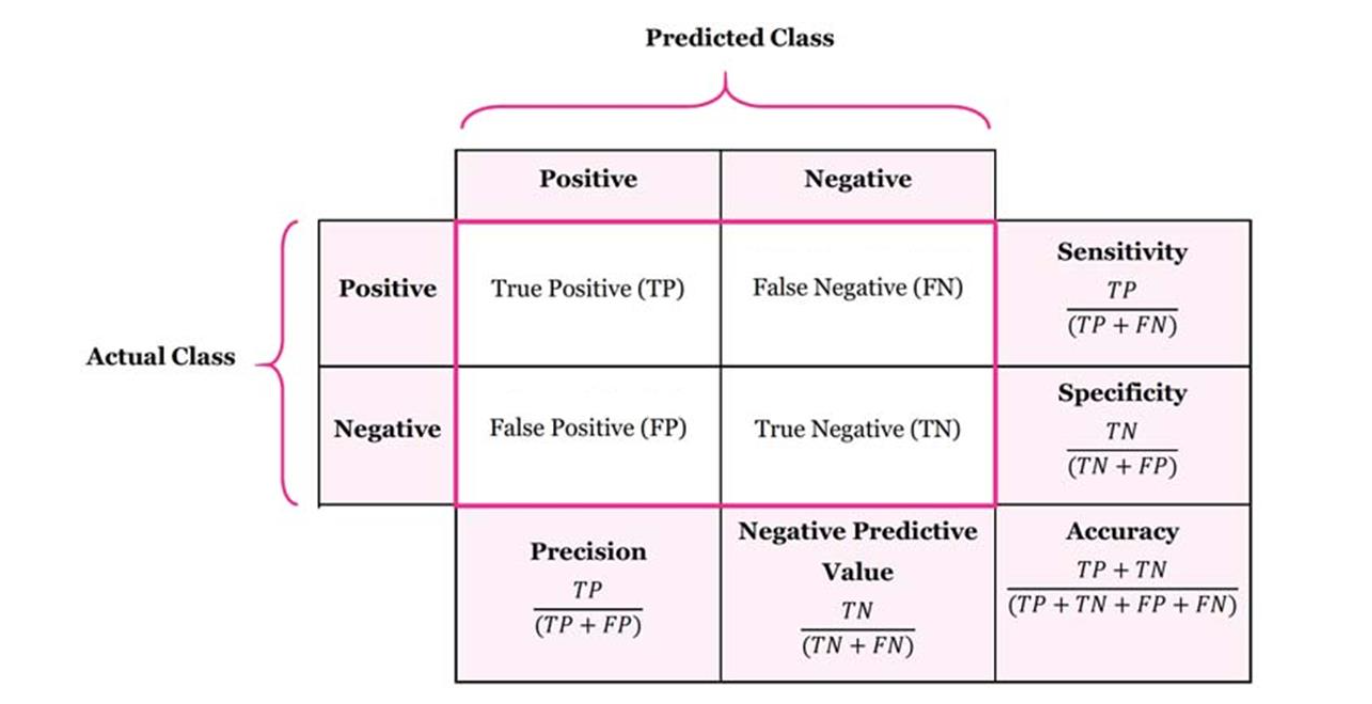
\includegraphics[scale=0.5]{images/conf.png}
\end{center}


\subsection{Multiclass Classification}
\begin{itemize}
\item Requires minor changes to our PyTorch implementation:
\begin{enumerate}
\item The final output layer has as many neurons as classes.
\item Apply the softmax activation function on the final layer to obtain class probabilities
\item Use the multiclass cross-entropy loss function
\end{enumerate}
\item Softmax function calculates the probabilities distribution of the event over ‘k’ different events.
\begin{itemize}
\item Calculates the probabilities class over all possible classes.
\item The range will be 0 to 1, and the sum of all the probabilities will be equal to one.
\end{itemize}
\end{itemize}
$$ \sigma (z) _j = \frac{e^z_j}{\sum_{k=1}^K e^z_k} \quad \quad \text{for        } j = 1, \cdots, k$$

\pagebreak



\section{Convolutional Neural Networks (CNNs)}
\hrule \vspace{15pt}

\subsection{Large Networks}
\begin{itemize}
\item Using a large fully connected layer could be problematic
\begin{itemize}

\item Computing predictions (forward pass) will take longer
\item A large number of weights requires a lot of training data to avoid overfitting (exponential relationship)
\item Small shift in image can result in large change in prediction (each pixel would be multiplied by a different weight)
\item Does not make use of the geometry of the image
\end{itemize}
\end{itemize}

\subsection{Convolutional Filters}
\begin{itemize}
\item People have used the idea of convolutional filters in computer vision even before the rise of machine learning.
\item They hand-coded filters that can detect simple features, for example to detect edges in various orientations.
\item Computing the convolution of image $I$ with filter $K$
\begin{enumerate}
\item Flip rows and columns of kernel
\item Multiply each pixel in range of kernel by the corresponding element of flipped kernel, sum all these products and write to a new 2d array; essentially a dot product 
\item Slide kernel across all areas of the image until you reach the ends; optional,  can use zero padding to maintain size of output
\end{enumerate}
\end{itemize}
\begin{figure}[H]
\begin{center}
\subfigure
{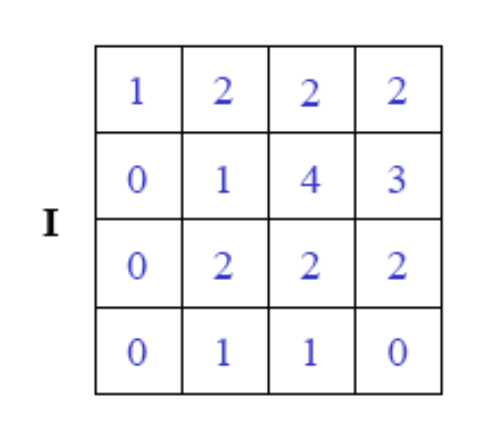
\includegraphics[width=3cm]{images/I.png}}
\subfigure
{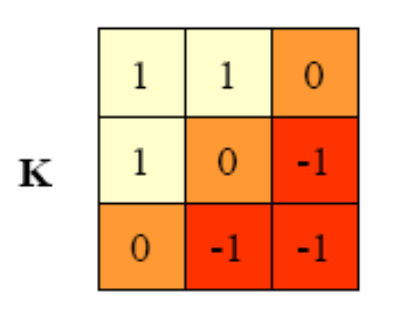
\includegraphics[width=3cm]{images/K.png}}
\end{center}
\end{figure}

\subsection{Convolutional Neural Networks}
\begin{itemize}
\item We can introduce convolutional filters into our neural network so that we don’t have to hand craft the features
\item Locally-connected layers: look for local features in small regions of the image
\item Weight-sharing: detect the same local features across the entire image
\item Neural Network learns the kernel values (or weights)
\item Two types of layers: \textbf{convolution} and \textbf{pooling}
\item Can express the output dimension as 
$$ n_{i+1} = \frac{n_i + 2p-f}{s} + 1 $$
\end{itemize}

\begin{center}
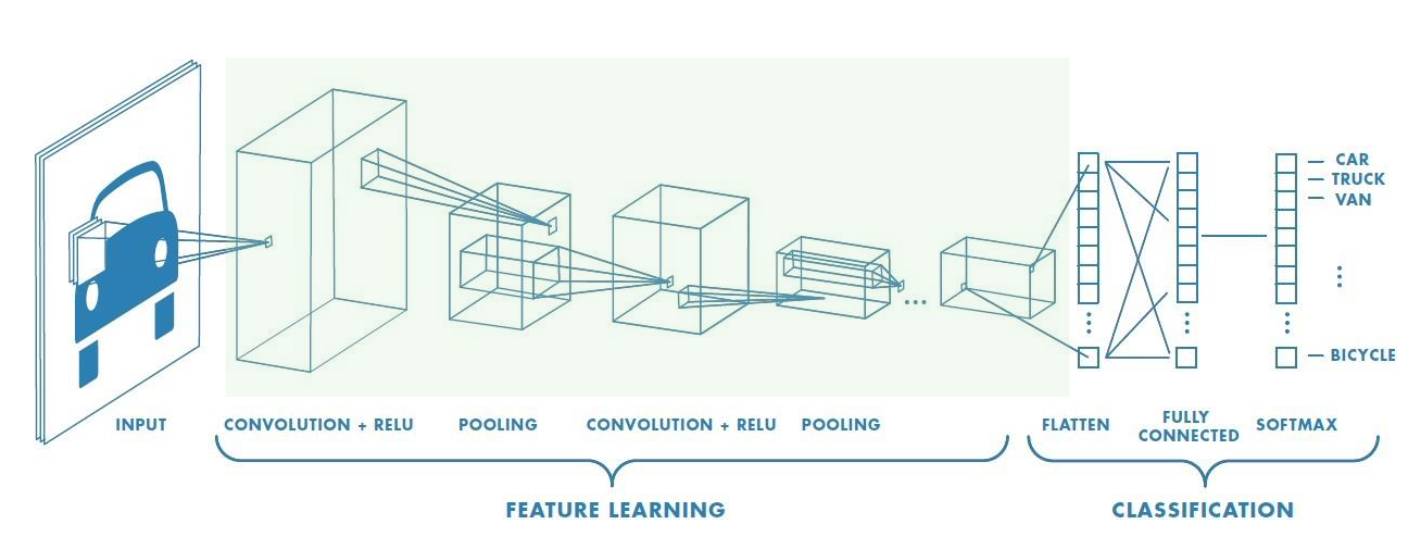
\includegraphics[scale=0.6]{images/cnn.png}
\end{center}

\subsection{Pooling Layers}
\begin{itemize}
\item Dimensionality reduction (downsampling) is achieved using pooling layers
\item Performed independently along the depth of a tensor
\item Max pooling is the most common choice for pooling
\item No parameters to learn!
\end{itemize}

\subsection{Deeper CNN Architectures}
\begin{itemize}
\item \textbf{LeNet}
\begin{itemize}
\item First introduced by Yann LeCun in 1989
\item 7 layers
\item 60,000 parameters to learn
\end{itemize}
\item \textbf{AlexNet}
\begin{itemize}
\item Won ImageNet competition in 2012 with 15.3 \% error rate
\item 60 million parameters
\item Over 90 epochs and 6 days of training
\item Can be implemented with transfer learning
\end{itemize}
\item \textbf{Inception}
\begin{itemize}
\item Won ImageNet competition in 2014 with 6.67 \% error rate (close to human level performance)
\item 22 layer deep
\item Parameters reduced from 60 million to 4 million
\end{itemize}
\item \textbf{VGG} 
\begin{itemize}
\item Runner up at ImageNet competition in 2014
\item Initially 16 convolutional layers, then 19
\item 138 million parameters which can be challenging to handle
\end{itemize}
\item \textbf{ResNet}
\begin{itemize}
\item Won ImageNet competition in 2015 with 3.57 \% error rate (better than human level performance)
\item 152 layers
\end{itemize}
\end{itemize}

\subsection{CNN Limitations}
\begin{itemize}
\item Dependent on data
\begin{itemize}
\item Scale invariance
\item Rotation invariance
\item Translation invariance
\end{itemize}
\item They do not code position and orientation into their predictions
\begin{itemize}
\item The final label of an image or the final prediction of the CNN is position invariant.
\item CNN should be able to identify the image as being small, large or upside down and it should have an internal representation of the position of that face.
\item Take an image and create many versions of it by tilting it, inverting it, rotating it and so on (\textbf{Image Augmentation})
\item This helped CNNs to learn an internal representation of an image with many different viewpoints.
\end{itemize}
\item Point of reference is not tracked
\item Hyperparameter tuning is not trivial
\item Convolution is computationally expensive
\item Require large datasets
\end{itemize}



\pagebreak



\section{Autoencoders}
\hrule \vspace{15pt}

\subsection{Unsupervised Learning}
\begin{itemize}
\item There are some challenges with supervised learning
\begin{itemize}
\item Requires large amounts of labeled data
\item Obtaining labeled data is expensive
\item Often there is a lot more unlabeled data than labeled.
\item Not what we see in biology
\end{itemize}
\item Our brains are constantly observing the world around us for patterns, or some structure to relate objects.
\item Patterns or clusters of similar features can tell us a great deal about the data before we even have a label.
\end{itemize}

\subsection{Autoencoder Overview}
\begin{itemize}
\item Find efficient representations of input data that could be used to reconstruct the original images.
\item Composed of two parts:
\begin{itemize}
\item \textbf{Encoder} converts the inputs to an internal
representation (dimensionality reduction)
\item \textbf{Decoder} converts the internal representation to the outputs (generative network)
\end{itemize}
\item Applications include:
\begin{itemize}
\item Feature Extraction
\item Unsupervised Pretraining
\item Dimensionality Reduction
\item Generate new data
\item Anomaly detection
\end{itemize}
\end{itemize}

\subsection{Autoencoder Architecture}
\begin{itemize}
\item Typically the number of outputs is the same as the inputs
\item Hour glass shape creating a bottleneck layer or lower dimensional representation
\item Not used for supervised learning.  The task is not to predict something about the data!
\item It is forced to learn the most important features in the input data and drop the unimportant ones
\item Potential for Overfitting!
\begin{itemize}
\item If encoder is too deep it could map each
input to a single arbitrary number
\item Such an encoder would reconstruct the training data perfectly and would not have learned any useful representations
\item Unlikely to generalize to new instances.
\end{itemize}
\item One way to ensure that an autoencoder is properly trained is to compare the inputs and the outputs.
\item Noise can be added to the input images of the autoencoder to force it to learn useful features; prevents the autoencoder from trivially copying its inputs to its outputs, has to find patterns in the data.
\end{itemize}


\subsection{Convolutional Autoencoder}
\begin{itemize}
\item The autoencoders mentioned up until now did not take advantage of spatial information
\item Adding convolutional layers can add improvements when trying to generate image data
\item The encoder works with convolution layers (pooling layers optional).
\item The decoder tries to mirror the encoder but instead of "making everything smaller" it has the goal of "making everything bigger" to match the original size of the image --- use  \textbf{Transposed Convolution}:
\begin{enumerate}
\item Take each pixel of your input image
\item Multiply each value of your kernel with the input pixel to get a weighted kernel 
\item Insert this in your output to create an image
\item Sum the outputs where they overlap
\end{enumerate}
\end{itemize}

\begin{center}
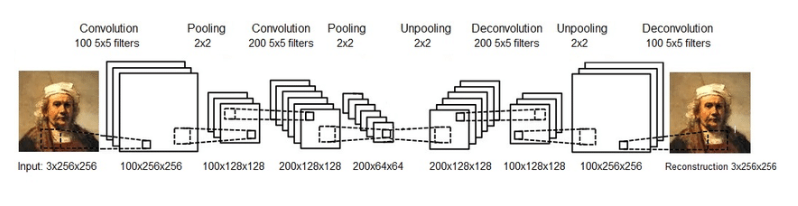
\includegraphics[scale=1.2]{images/auto.png}
\end{center}


\pagebreak

\section{Recurrent Neural Networks (RNNs)}
\hrule \vspace{15pt}

\subsection{One-Hot Encoding}
\begin{itemize}
\item For word (or categorical data) where there is no order, integer encoding is not enough.
\item A better way... convert word features into numerical features with one-hot encoding. 
\item Some advantages/disadvantages
\begin{itemize}
\item Dimensions grow with number of words
\item One-hot encoding assumes each word is completely independent
\end{itemize}
\end{itemize}

\subsection{Word Embeddings}
In order to talk about which words have “similar” GloVe embeddings, We need to introduce a measure of distance in the embedding space.

\subsubsection{Euclidean Distance}
The Euclidean distance of two vectors $x = [x_1, x_2, \cdots, x_n]$ and $y = [y_1, y_2,  \cdots, y_n]$ is the 2-norm of their difference $x-y$:
$$\sqrt{\sum_i (x_i - y_i)^2}$$
\subsubsection{Cosine Similarity}
The cosine similarity of two vectors $x$ and $y$ is the cosine of the angle between the two vectors.  Cosine similarity is useful when we want a distance measure that is invariant to the magnitude of the vectors.
\begin{center}
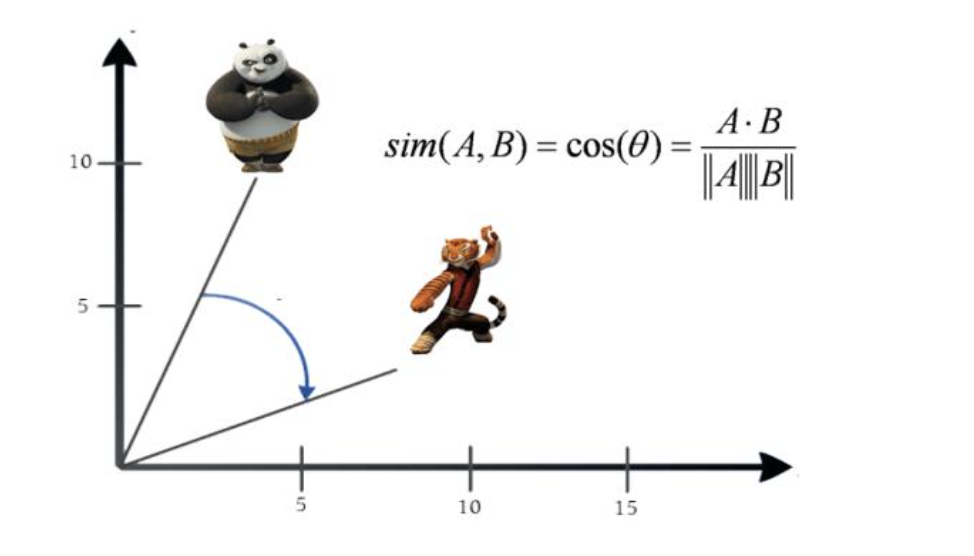
\includegraphics[scale=0.7]{images/cosine.png}
\end{center}

\subsection{RNN Architecture}
\begin{itemize}
\item Can take in variable-sized sequential input 
\item Can remember things over time, or has some sort of memory or state
\item General procedure :
\begin{enumerate}
\item Start with an initial hidden state with a blank slate (can be a vector of all zeros) 
\item Hidden state is updated based on previous hidden state, and the input using the same neural network as before (weight sharing)
\item Continue updating the hidden state until we run out of tokens.
\item Use the last hidden state as input to a prediction network
\end{enumerate}
\item The forward path in RNNs shares similarities with the a fully-connected neural network
\item Weights applied on input and hidden state
\end{itemize}

\begin{center}
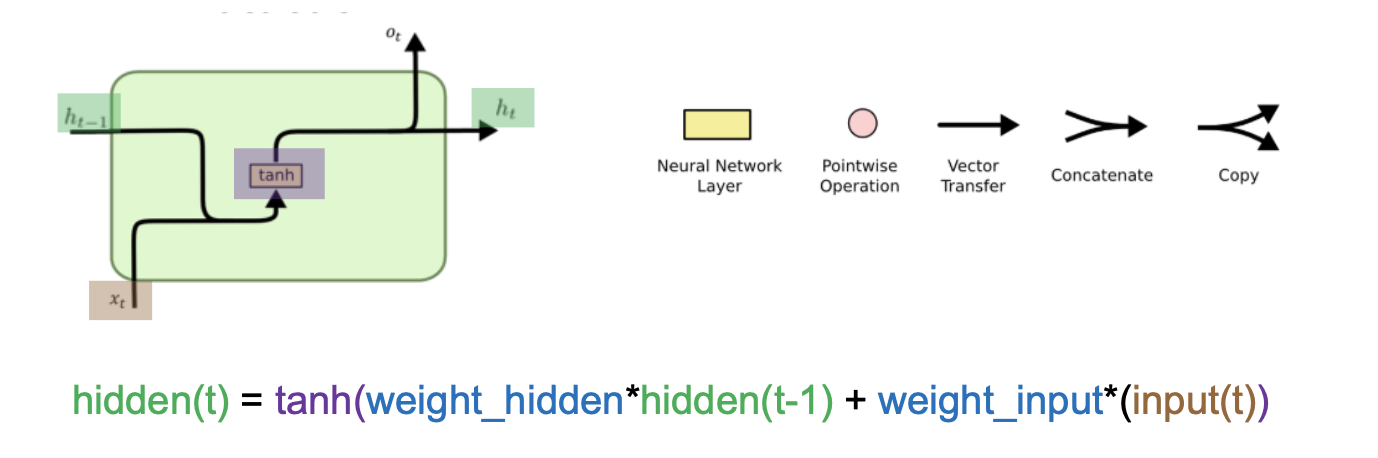
\includegraphics[scale=0.5]{images/rnn.png}
\end{center}

\subsection{Long Term Dependencies}
\begin{itemize}
\item RNNs historically hard to train; good for capturing recent information, but difficulties with long-term dependencies
\item \textbf{Long Short-Term Memory (LSTM) networks}
\begin{itemize}
\item take advantage of an extra hidden state referred to as the cell state
\item gates to manage long-term memory and regulate vanishing/exploding gradients
\item adds more complexity
\end{itemize}
\end{itemize}

\begin{center}
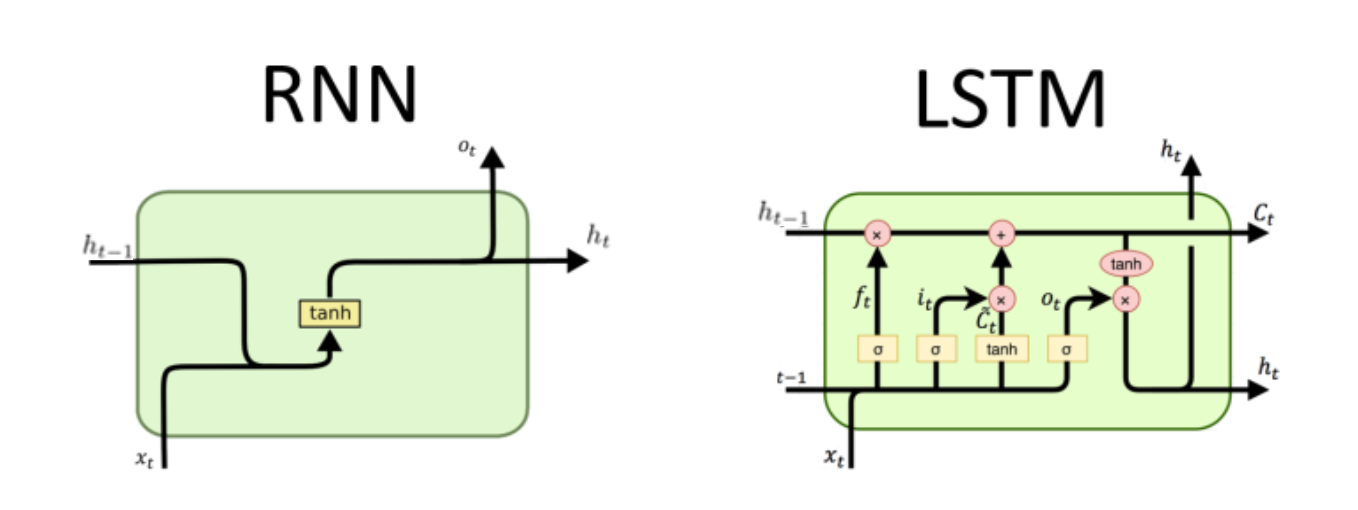
\includegraphics[scale=0.4]{images/compare.png}
\end{center}
\begin{center}
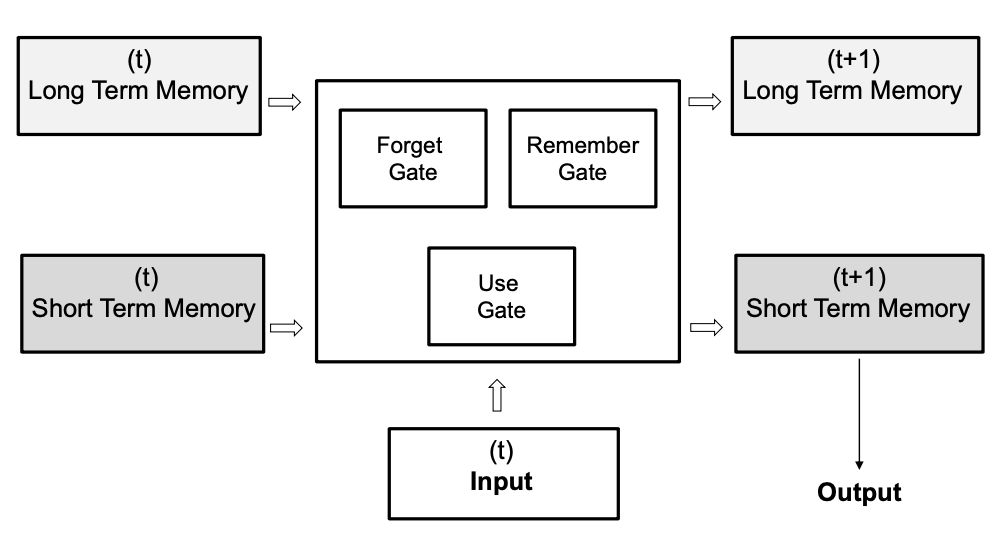
\includegraphics[scale=0.7]{images/lstm.png}
\end{center}
\begin{itemize}
\item \textbf{Gated Recurrent Units (GRUs)}
\begin{itemize}
\item Variant on LSTM
\item Introduced in 2014, it combines gates and
merges cell state and hidden state
\item It is much simpler to implement and faster than standard LSTM
\end{itemize}
\end{itemize}
\begin{center}
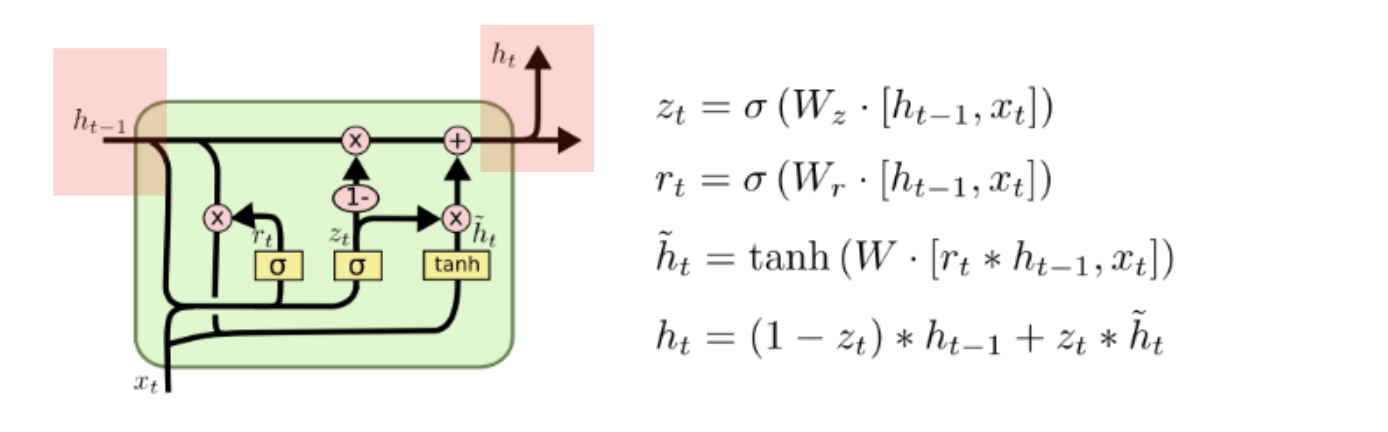
\includegraphics[scale=0.5]{images/gru.png}
\end{center}

\subsection{Generative RNNs}
\begin{itemize}
\item Learning to generate new sequences will require some changes:
\begin{itemize}
\item Input sequence representation --- start and end token
\item Training-time behaviour --- teacher-forcing
\item Test-time behaviour --- sampling and temperature
\end{itemize}
\item\textbf{ RNN For Prediction:}
\begin{itemize}
\item Process tokens one at a time
\item Hidden state is a representation of all the tokens read thus far
\end{itemize}
\item \textbf{RNN For Generation:}
\begin{itemize}
\item Generate tokens one at a time
\item Hidden state is a representation of all the tokens to be generated
\end{itemize}
\end{itemize}
\begin{itemize}
\item Process:
\begin{itemize}
\item $token = preprocess (input)$
\item $hidden = update\_function (hidden, token)$
\item $token\_distribution = prediction\_function (hidden)$
\item $token = sample\_from (token_distribution)$
\end{itemize}
\end{itemize}
\begin{center}
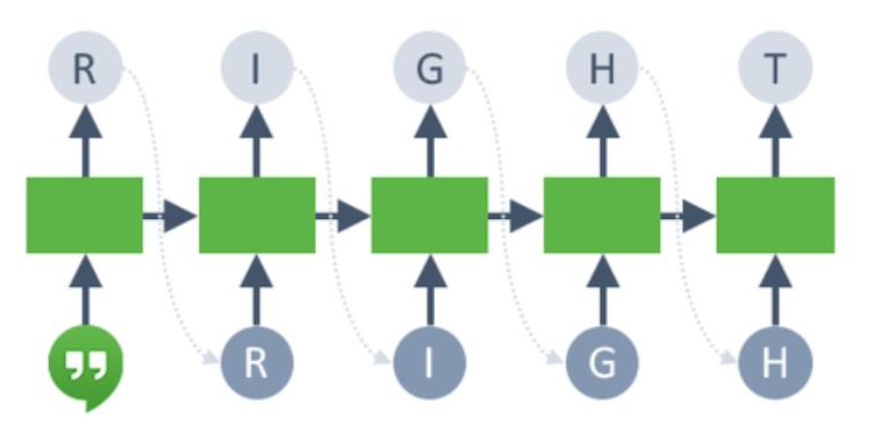
\includegraphics[scale=0.6]{images/gen.png}
\end{center}


\pagebreak

\section{Generative Adversarial Networks (GANs)}
\hrule \vspace{15pt}

\subsection{Generative Models}
\begin{itemize}
\item Learns the structure of a set of input data, and can be used to generate new data
\item \textbf{examples}: Autoencoders, RNNs for text generation
\end{itemize}

\subsection{GAN Architecture}
\begin{itemize}
\item The idea is to train two networks
\begin{itemize}
\item \textbf{Generator Network}: try to fool the discriminator by generating real-looking images
\begin{itemize}
\item Input: A random noise vector
\item Output: A generated image
\end{itemize}
\item \textbf{Discriminator Network}: try to distinguish between real and fake images
\begin{itemize}
\item Input: An image
\item Output: A binary label (real or fake)
\end{itemize}
\end{itemize}
\item The loss function of the generator (the model we care about) is defined by the discriminator! 
\item Applies a minimax strategy
\begin{itemize}
\item the discriminator will try to do the best job it can
\item the generator is set to make the discriminator as wrong as possible
\end{itemize}
\end{itemize}

\begin{center}
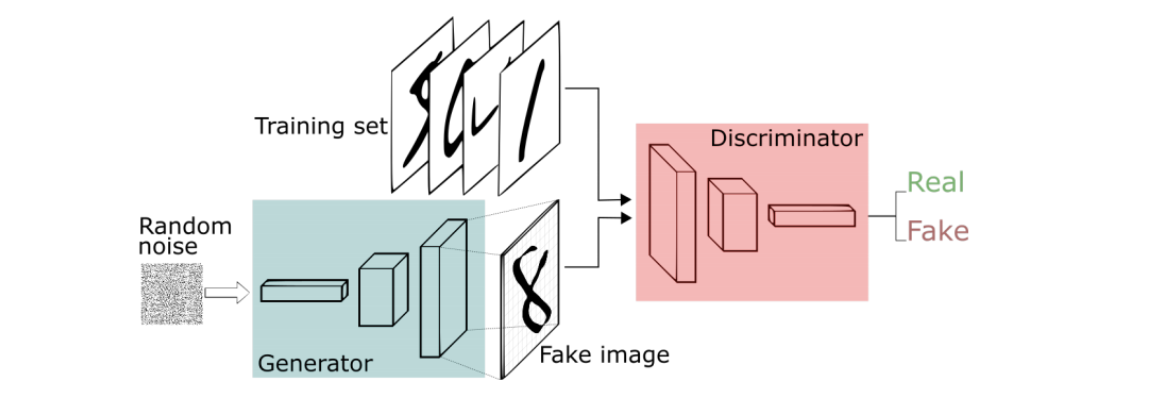
\includegraphics[scale=0.9]{images/gan.png}
\end{center}

\subsection{Loss Function}
\begin{itemize}
\item Tune \textbf{discriminator} weights to maximize the probability that the ...
\begin{itemize}
\item discriminator labels a real image as real
\item discriminator labels a generated image as fake
\end{itemize}
\item Tune \textbf{generator} weights to maximize the probability that the ...
\begin{itemize}
\item discriminator labels a generated image as real
\end{itemize}
\end{itemize}

\subsection{Adversarial Attack}
\begin{itemize}
\item \textbf{Goal} - choose a small perturbation $\epsilon$ on an image $x$ so that a neural network $f$ misclassifies $x+ \epsilon$
\item \textbf{Approach} - use the same optimization process to choose $\epsilon$ to minimize the probability that
$$ f(x+ \epsilon ) = correct \; class $$
\item Treating $\epsilon$ as the parameters
\item \textbf{Non-Targeted Attack} - minimize the probability that $ f(x+ \epsilon ) = correct \; class $
\item \textbf{Targeted Attack} - maximize the probability that $ f(x+ \epsilon ) = targeted \; class $
\item \textbf{White Box} - assumes the model is known,  we need to know the architectures and weights of $f$ to optimize $\epsilon$
\item \textbf{Black Box} - don’t know the architectures and weights of $f$ to optimize $\epsilon$; substitute model mimicking target model with known,  differentiable function
\end{itemize}

\pagebreak

\section{Reinforcement Learning}
\hrule \vspace{15pt}

\subsection{Overview}
\begin{itemize}
\item Reinforcement learning is different from supervised learning
\begin{itemize}
\item There is no supervision - only a scalar reward signal 
\item There is a notion of "time" (steps/moves)
\item Feedback is delayed, not instantaneous 
\item Decisions/actions will affect the subsequent data received
\end{itemize}
\item There are two key components 
\begin{itemize}
\item \textbf{Environment} - provides the agent with the current state and provides a reward at each time step (mostly 0 reward)
\item \textbf{Agent} - chooses an action at each time step, given the state
\end{itemize} 
\begin{center}
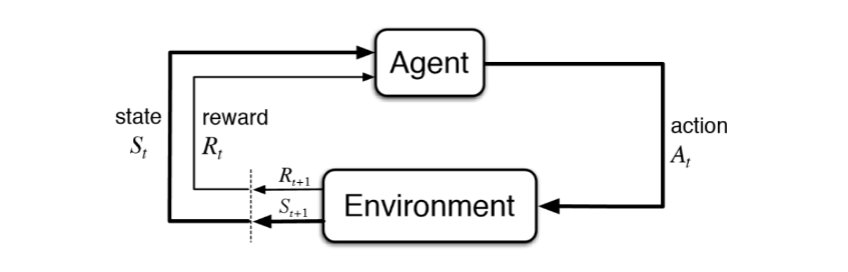
\includegraphics[scale=0.9]{images/rl.png}
\end{center}\
\end{itemize}

\subsection{Rewards}
\begin{itemize}
\item A \textbf{reward} $R_t$ is a scalar feedback signal
\item The goal of the agent is to select actions to maximize total future reward.
\item Setting up rewards to get good agent behaviour is tricky, If the reward is not well designed, it can lead to reward hacking
\item Two types of rewards:
\begin{itemize}
\item \textbf{Sparse Reward} - there is a nonzero reward in only a few time steps (\textit{i.e. win/loss at the end})
\item \textbf{Dense Reward} - there is a nonzero reward in most time steps (\textit{i.e. some form of score})
\end{itemize}
\end{itemize}

\subsection{Major Components}

\subsubsection{Agent}
\begin{itemize}
\item algorithm that makes the decision on what action to take
\item can contain machine learning algorithms that learn one or more of the policy, value function, or model.
\item two main types:
\begin{itemize}
\item \textbf{Value Based Agent }- learn value function only; choose the action that maximize the value function of the next state
\item \textbf{Policy Based Agent }- learn policy function only (no estimate of value function)
\end{itemize}
\end{itemize}
\subsubsection{Policy}
\begin{itemize}
\item the agent's behaviour, the action it chooses at a state.  
\item usually represented with the letter $\pi$
\item a function that maps state to action
\begin{itemize}
\item \textbf{deterministic:} $ a = \pi(s)$
\item \textbf{stochastic}: $\pi (a | s) = P(A_t = a | S_t = s )$
\end{itemize}
\item can parameterize $\pi$ using a neural network
\end{itemize}
\subsubsection{Value Function}
\begin{itemize}
\item a prediction of future reward,  assuming we follow a particular policy
\item used to evaluate the goodness or badness of states
\item the value function is a function that maps state to expected discounted return
\end{itemize}
\subsubsection{Q-Function}
\begin{itemize}
\item maps (state, action) pairs to expected discounted return
\item can parameterize the Q-function using a neural network
\end{itemize}
\subsubsection{Model}
\begin{itemize}
\item predicts what the environment will do next
\begin{itemize}
\item predict the next state (given the current state and an action to take)
\item predict the next reward
\end{itemize}
\end{itemize}

\subsection{Value Iteration Algorithm }
\begin{enumerate}
\item For all $s$ set $V(s) = 0$
\item Repeat until convergence:
\begin{enumerate}
\item For all actions, $a$ , determine and set $Q(s,a)$
\item $V(s) = \max_a Q(s,a)$
\end{enumerate}
\item Return $Q$
\end{enumerate}
$$ Q(s,a) = \sum_{s} T(s,a,s') \cdot [R(s,a,s')+ \gamma \cdot V(s')]$$
\begin{itemize}
\item $T(s, a, s')$ is the transition probability from state $s$ to state $s'$, given that the agent chose action $a$
\item $R(s, a, s')$ is the immediate reward that the agent gets when it goes from state $s$ to state $s'$, given that the agent chose action $a$
\item $\gamma$ is the discount rate
\end{itemize}
 
\subsection{Q-Learning Algorithm }
\begin{enumerate}
\item For all $s$ set $ Q(s,a) = 0,$ and $V(s) = 0$
\item Repeat until convergence:
\begin{enumerate}
\item Randomly select state $s$ and randomly select action $a$ from available actions at state $s$
\item If immediate reward available update matrix $R(s,a)$
\item Update $Q(s,a)$
\item $V(s) = \max_a Q(s,a)$
\end{enumerate}
\item Return $Q$
\end{enumerate}
$$ Q(s,a) =(1-\alpha)\cdot Q(s,a) + \alpha \cdot [R(s,a,s')+ \gamma \cdot V(s')]$$

\subsection{Exploration vs Exploitation}
\begin{itemize}
\item \textbf{Exploitation}: Take actions the function already thinks will lead to a good outcome
\item \textbf{Exploration}: Try making novel actions and see if you discover a way to adjust the function to get even better outcomes
\end{itemize}



\pagebreak

\section{Ethics and Fairness}
\hrule \vspace{15pt}

\subsection{What is Ethics?}
\begin{itemize}
\item Ethics deals with moral principles that govern a person's behavior or the conducting of an activity
\item Ethics in AI is primarily focused on social, political and cultural impact of the application of AI software
\end{itemize}
\subsection{Convergence of Ethical Principles}
\begin{itemize}
\item Transparency
\item Justice and Fairness 
\item Non-Maleficence
\item Responsibility
\item Privacy
\end{itemize}
\subsection{Causes of Bias}
\begin{itemize}
\item \textbf{Skewed Sample:} If by chance bias is introduced,then such bias may compound over time: future observations confirm prediction and fewer opportunity to make observations that contradict prediction. 
\item \textbf{Tainted Examples: }Human bias can be captured by the model.
\item \textbf{Limited Features: }Minority groups data may have less information, or unreliably collected data. System tends to have much lower accuracy for the prediction of the minority group.
\item \textbf{Sample Size Disparity: }When there is much less training data coming from the minority group than those from the majority group. Model has less information to accurately model the minority group.
\item \textbf{Proxies:} Excluding sensitive attributes such as race/gender may not be enough. Other features such as neighbourhood could act as proxies of sensitive attribute. Can be difficult to decide if we should include feature or not. 
\end{itemize}

\subsection{Defining Fairness}
\subsubsection{Disparate Treatment }
\begin{itemize}
\item Model suffers from disparate treatment if decisionsare correlated with the subject’s sensitive attribute.
\item For example, in the sentencing model, does the model treat people of different ethnicities similarly?
\end{itemize}
\subsubsection{Disparate Impact}
\begin{itemize}
\item Model suffers from disparate impact if decisions disproportionally hurt (or benefit) people with sensitive attributes
\item For example, suppose we are building a model to determine whether or not an applicant is admitted to graduate school.
\end{itemize}

\subsection{Measuring Fairness }
\subsubsection{Demographic Parity }
\begin{itemize}
\item Acceptance ratesof applications from both groups must be equal
\item \textbf{Problem}: Fairness is measured at a group level; 
model can hire qualified people from one group, and random people from the other
\end{itemize}
\subsubsection{Equalized Odds }
\begin{itemize}
\item Model should be equally accurate across both groups
\item Also known as “accuracy parity”
\item \textbf{Problem}: False positives and false negatives have different impacts; does not help to close the gap between the two groups
\end{itemize}
\subsubsection{Individual Fairness }
\begin{itemize}
\item Similar individuals from different groups should be treated similarly
\item \textbf{Problem}: Hard to determine appropriate measure of “similarity” of inputs
\end{itemize}

\subsection{Increasing Fairness}
\begin{itemize}
\item \textbf{Pre-processing:} remove information correlated to sensitive attributes
\item \textbf{Add regularization term:} add a “fairness” regularizer
\item \textbf{Post-processing:} change the way we use a model to make predictions
\end{itemize}

\end{document}
